\section{Machine Learning}

\begin{itemize}
\item What is machine learning?
\item Supervised learning, i.e.\ have labelled data.
\item Binary classification tasks: Every training example has a label indicating
  the class membership.
\item In HEP, the positive class is typically referred to as \emph{signal} while
  the negative class is referred to as \emph{background}.
\item What is training data, etc.
\item What is training.
\end{itemize}


\subsection{Boosted Decision Trees}

Boosted decision trees (BDT) are a classification algorithm consisting on an
ensemble of \emph{decision tree classifiers} that are combined to yield a more
powerful classifier. The ensemble of decision trees is created using a algorithm
referred to as \emph{boosting}, which iteratively constructs decision tree
classifiers while emphasising training examples that were incorrectly classified
in prior iterations. The following description of BDT focuses on the algorithm
implemented in \textsc{TMVA}~\cite{TMVA}, which is used in this thesis for the
training of BDTs.

Decision trees are the base classifiers used in BDTs. A decision tree partitions
a multivariate space by recursively performing binary splits along the
coordinate axes until a stopping criterion is met. The resulting binary tree
structure and partitioning is illustrated in \Cref{fig:decision_tree} for a
two-dimensional example. A decision tree with $n$~leaf nodes partitions the
multivariate space into $n$~disjoint subregions denoted by $R_i$ for
$i = 1, \dots, n$. The goal of decision tree learning is to find a partitioning
such that the resulting subregions have low impurity, that is, the regions are
mostly populated by training example of a single class. The impurity of a tree
node is quantified by the Gini index
\begin{align*}
  I_{\text{G}}(p) = 2 p (1 - p) \,\text{,}
\end{align*}
where $p$ is the proportion/purity of positive class in a given
node~\cite{hastie09}. Decision trees are typically grown using a \emph{greedy}
strategy by splitting nodes such that the weighted sum of Gini impurities of the
resulting daughter nodes is minimised, where the impurities are weighted
according to the total weight of training examples populating a given node.



Probabilistic classification:

Majority voting:



\begin{figure}[htbp]
  \centering

  \begin{subfigure}[b]{0.46\textwidth}
    \centering
    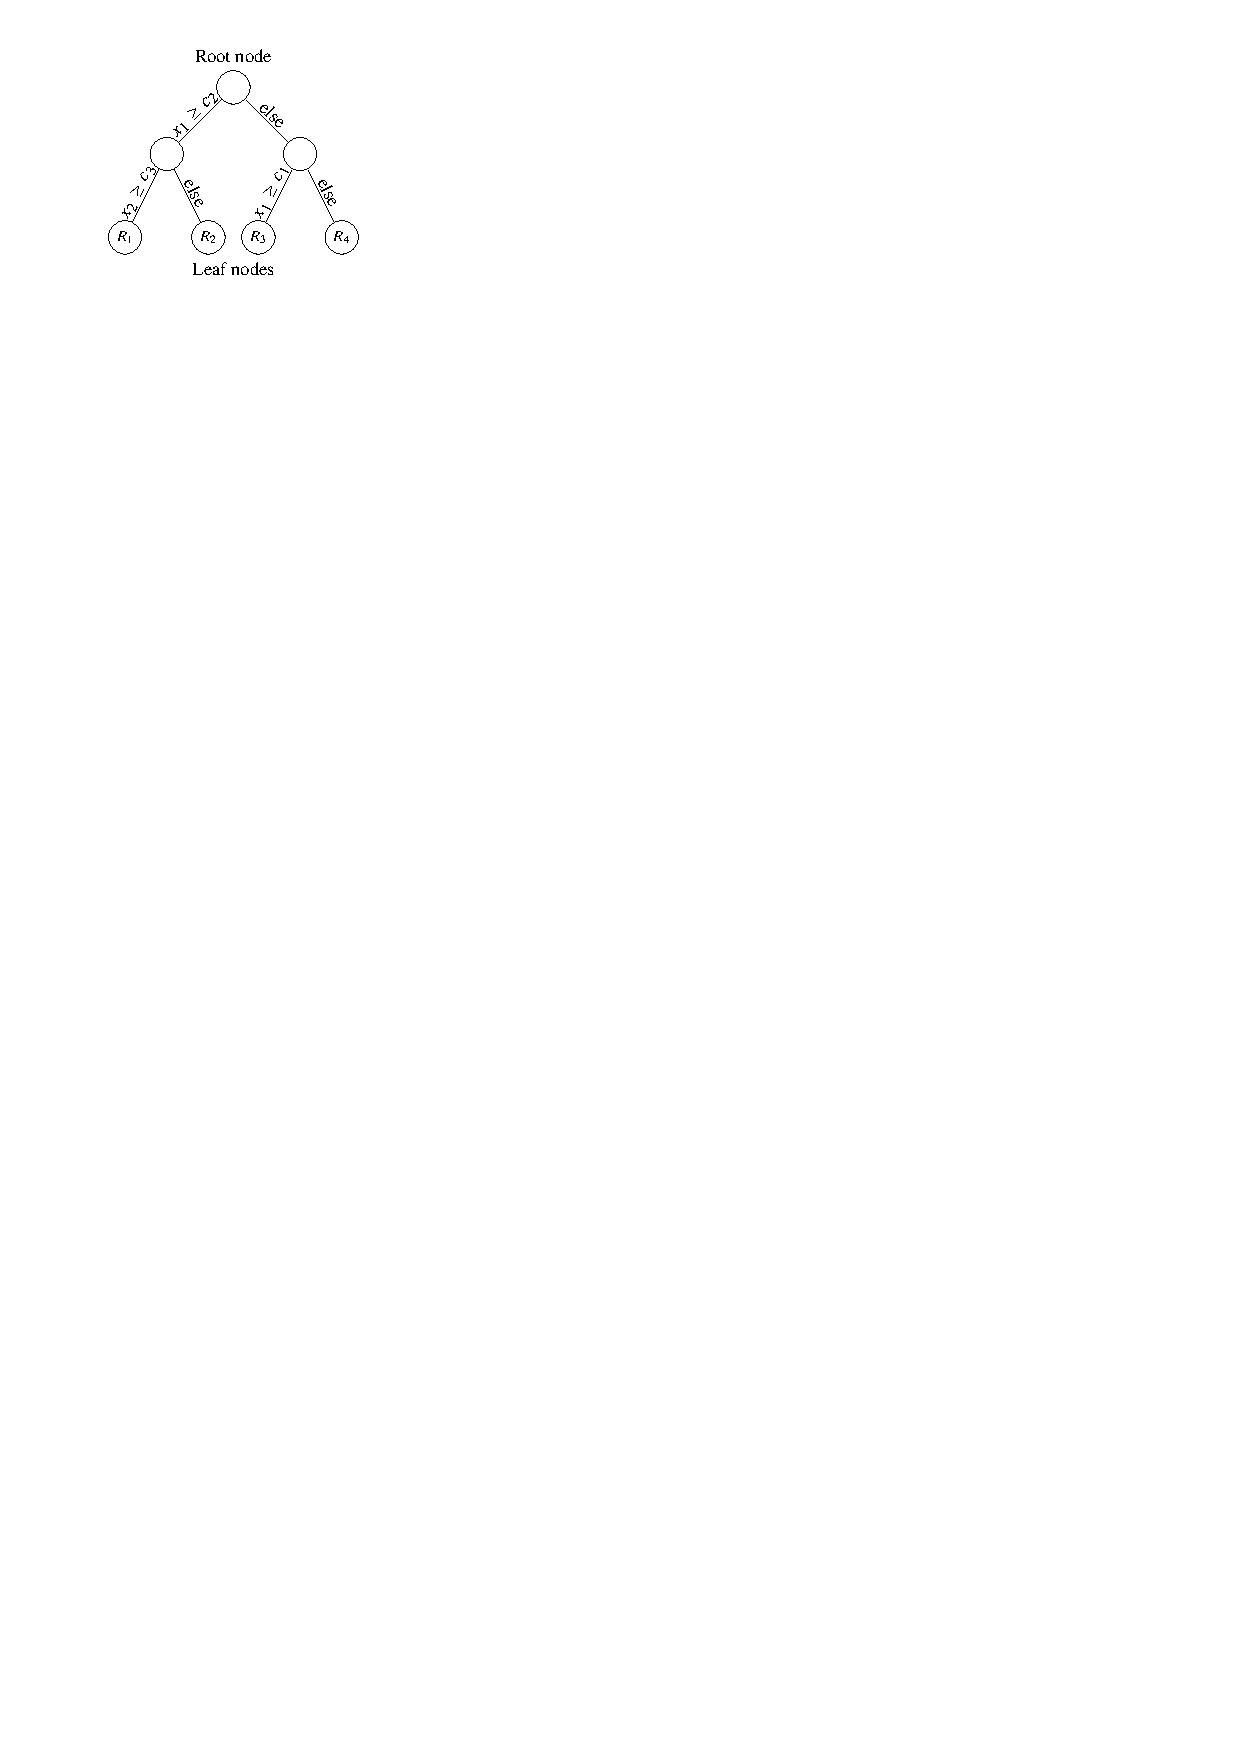
\includegraphics[scale=1.05]{ml/decision_tree}
    \caption{Binary tree structure of a decision tree.}
  \end{subfigure}\hfill%
  \begin{subfigure}[b]{0.46\textwidth}
    \centering
    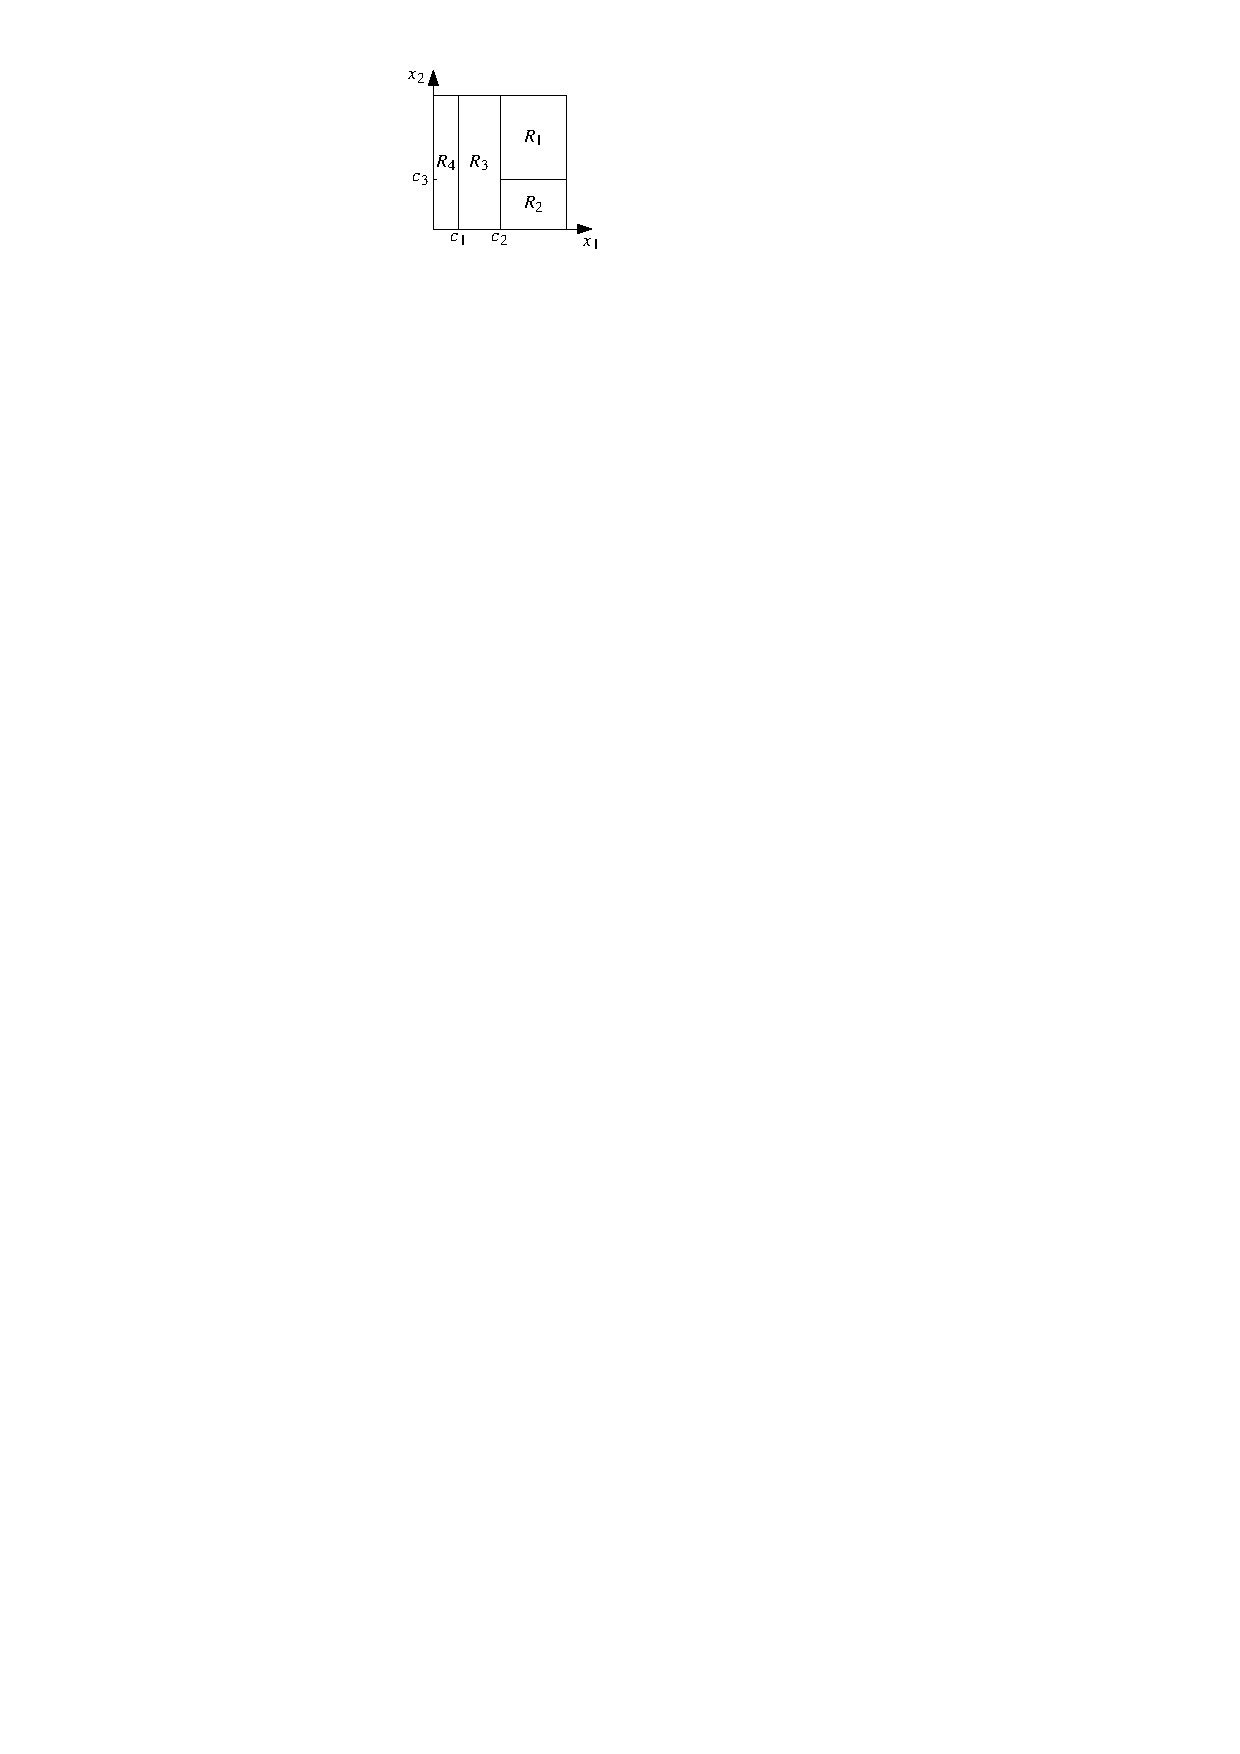
\includegraphics[scale=1.05]{ml/decision_tree_partitioning}
    \vspace*{0.7em}
    \caption{Partitioning resulting from the binary tree in (a).}
  \end{subfigure}\hfill%

  \caption{Example of a decision tree in a two-dimensional space with
    coordinates $(x_1, x_2)$. The tree has a depth of two resulting in four leaf
    nodes that define the regions $R_1, \dots, R_4$. The figure is adapted from
    Ref.~\cite{hastie09}.}%
  \label{fig:decision_tree}
\end{figure}

Booooooooostiiing... yeah!


\subsection{Neural Networks}

\subsubsection{Recurrent Neural Networks}%
\label{sec:rnn}


%%% Local Variables:
%%% mode: latex
%%% TeX-master: "../../phd_thesis"
%%% End:
